\documentclass{article}
\usepackage[T1]{fontenc}

\usepackage{float}
\usepackage{aliascnt}
\newaliascnt{eqfloat}{equation}
\newfloat{eqfloat}{h}{eqflts}
\floatname{eqfloat}{Equation}

\newcommand*{\ORGeqfloat}{}
\let\ORGeqfloat\eqfloat
\def\eqfloat{%
  \let\ORIGINALcaption\caption
  \def\caption{%
    \addtocounter{equation}{-1}%
    \ORIGINALcaption
  }%
  \ORGeqfloat
}
\usepackage{siunitx} % Provides the \SI{}{} and \si{} command for typesetting SI units
\usepackage{graphicx} % Required for the inclusion of images
\usepackage{natbib} % Required to change bibliography style to APA
\usepackage{amsmath} % Required for some math elements 
\usepackage[portuges]{babel}
\usepackage[utf8]{inputenc}
\usepackage{longtable}
\usepackage[table,xcdraw]{xcolor}
\usepackage{caption}
\usepackage{subcaption}
\setlength\parindent{0pt} % Removes all indentation from paragraphs

\renewcommand{\labelenumi}{\alph{enumi}.} % Make numbering in the enumerate environment by letter rather than number (e.g. section 6)

%\usepackage{times} % Uncomment to use the Times New Roman font

%----------------------------------------------------------------------------------------
%	DOCUMENT INFORMATION
%----------------------------------------------------------------------------------------

\title{Avaliação de métodos estocásticos aplicados à problemas de minimização da Energia Potencial Total de sistemas mecânicos}

\author{Luis Vinicius Costa Silva}
\date{\today}
\begin{document}
\maketitle
\nocite{*} 
\begin{center}
\begin{tabular}{l r}
Disciplina: & Sistemas Bioinspirados \\
Professor: & Fran Sérgio lobato
\end{tabular}
\end{center}
\abstract
O estado de equilíbrio de um sistema mecânico (ou de qualquer outro sistema clássico) pode ser obtido através da minimização de uma função objetivo que relacione os campos de deslocamento do sistema a uma energia potencial total. A popularidade desta estratégia se justifica pelo fato da mesma necessitar apenas da primeira derivada e se utilizar de métodos de otimização já conhecidos. Este trabalho buscou avaliar dois algoritmos evolutivos (PSO e Evolução Diferencial) e um clássico (algoritmo de Powell) na resolução de dois problemas desta natureza. Notou-se que todos os métodos foram capazes de obter respostas dentro da faixa de tolerância estabelecida na maioria dos casos, sendo que a Evolução Diferencial se mostrou o melhor algoritmo estocástico, necessitando de menores populações e iterações para uma convergência aceitável.
\section{Introdução}
O Princípio do mínimo da Energia Potencial dita que o estado de equilíbrio mecânico de um sistema é aquele que (de todas as alternativas possíveis) tem a menor energia potencial (basicamente uma reformulação da segunda lei da Termodinâmica) (\cite{reddy2007introduction}). A determinação da configuração final de um sistema mecânico implica na formulação da função de energia potencial total do sistema em função das forças internas (energia armazenada por um sistema que sofre deformação - strain) e a energia potencial das forças externas. 
É sabido que a Energia Potencial Total de um sistema é dado pela diferença entre as forças internas (strain Energy/deformação) e o trabalho das Forças Externas.
\begin{equation}
\begin{split}
\pi = U + W
\end{split}
\end{equation}
Expandindo os termos da equação anterior, temos que:
\begin{equation}
\begin{split}
\pi = \sum_{e=1}^{n} \Lambda^{(e)} + \sum_{i=1}^{m} F_i u_i
\end{split}
\end{equation}

\begin{equation}
\begin{split}
\sum M_{A} = 0
\end{split}
\end{equation}


Onde $\ \Lambda^{(e)}$ é a energia de deformação para cada elemento do sistema e $F_i u_i$ é a força externa aplicada em cada campo de deslocamento do sistema.\newline
A energia potencial mínima do sistema pode ser obtida igualando a derivada da energia potencial pelo deslocamento a zero:
\begin{equation}
\begin{split}
\frac{\partial}{\partial u_i} \sum_{e=1}^n \Lambda^{(e)} + \frac{\partial}{\partial u_i} \sum_{i=1}^{m} F_i u_i = 0,\ i=1,2, ..., n
\end{split}
\end{equation}


O princípio do mínimo da Energia Potencial Total se faz útil pelo fato de ser computacionalmente mais rápido que uma integração de equação diferencial que representa a dinâmica do sistema, visto que são necessários computar estados intermediários do sistema até atingir o estado de equilíbrio, acarretando em mais uso de processamento e memória \cite{schlick1987powerful}. Além disso, a resolução deste tipo de problema por este princípio requer apenas a primeira derivada, além de incorporar as condição de contorno de força (condição de contorno natural,i.e: forças, momentos prescritos, etc.) automaticamente. O deslocamento
admissível precisa satisfazer somente a condição de contorno de deslocamento (condição de contorno geométrica) (\cite{hill1959some}) . \newline

Visto que tal diferenciação torna-se muito complicada para sistemas com vários $u_i$ (i.e: pontos de deslocamento), faz-se necessário a formulação do problema no formato de minimização, a fim de que algoritmos de otimização atinjam o resultado esperado \cite{felippa1977numerical}.

\section{Problemas de Teste}
Os problemas escolhidos são os de número 13 e 20 do capítulo 10 do livro "Numerical Methods in Engineering with Python 3" (\cite{kiusalaas2013numerical}). A escolha destes problemas se deu devido a facilidade em escrever e compreender a função objetivo e suas restrições, assim como a implementação de tais elementos na solução computacional. Além disso, ambos tem um grau de não-linearidade considerável, tornando um bom desafio para os métodos de otimização testados.\newline
O problema 2 possui restrições geométricas de igualdade, que foram implementadas na solução computacional através da reescrita da função objetivo utilizando o Método da Penalidade da Função Exterior (visto que os todos os algoritmos testados são de otimização irrestrita).
\subsection{Problema 1}
Considere o sistema abaixo:

\begin{figure}[H]
  \centering
  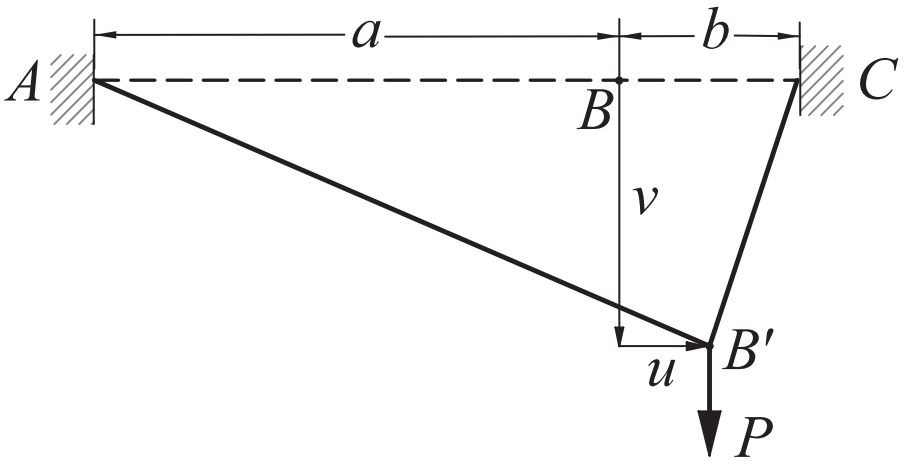
\includegraphics[width=0.5\linewidth]{problema_1.png}
  \caption{Diagrama do Problema 1}
\end{figure}

A corda elástica $A BC$ tem uma rigidez $k$. Quando a força vertical $P$ é aplicada em $B$, a corda é deformada para a forma $A B'C$. A energia potencial do sistema com esta característica de deformação é:

\begin{equation}
\begin{split}
\text{min}\text{\phantom{0}}V = & -Pv + \frac{k(a+b)}{2a} \delta_{AB} + \frac{k(a+b)}{2b} \delta_{BC} \phantom{0} \text{onde:} \\
\phantom{0} & \phantom{0} \\
\delta_{AB} = & \sqrt{(a+u)^2 + v^2} - a  \\
\delta_{BC} = & \sqrt{(b-u)^2 + v^2} - b  \\
\end{split}
\end{equation}

Busca-se o deslocamento $u$ e $v$ que minimizam a função de energia potencial total $V$, considerando:

\begin{itemize}
\item $a = 150\text{\phantom{0} mm}$;
\item $b = 50\text{\phantom{0} mm}$;
\item $k = 0.6\text{\phantom{0} N/mm}$;
\item $P = 5\text{\phantom{0} N}$
\end{itemize}

\subsection{Problema 2}
Considere o sistema abaixo:

\begin{figure}[H]
  \centering
  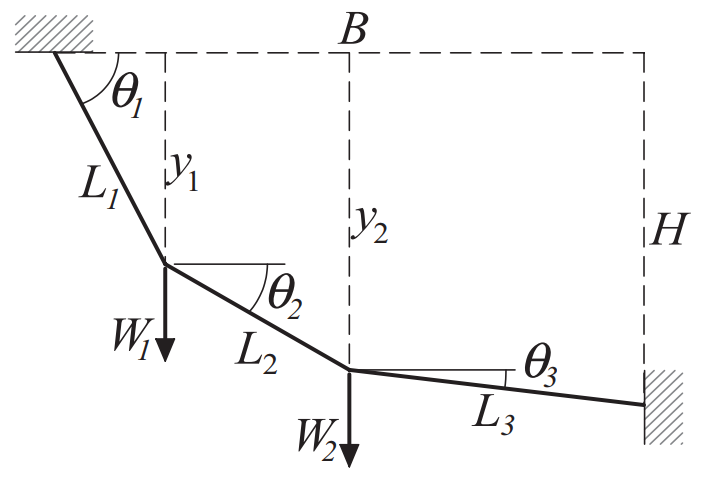
\includegraphics[width=0.5\linewidth]{problema_2.png}
  \caption{Diagrama do Problema 2}
\end{figure}

Como representado pelo figura acima, um cabo apoiado em suas extremidades suporta os pesos $W_1$ e $W_2$. A energia potencial total do sistema é dada por:

\begin{equation}
\begin{split}
V = & -W_1 y_1 - W_2 y_2 \\
\phantom{0} & \phantom{0} \\
\phantom{0} & \phantom{0} \\
\text{min\phantom{0}}V = & -W_1 L_1 \sin \theta_1 - W_2 (L_1 \sin \theta_1 + L_2 \sin \theta_2) \phantom{0}\text{s.t:} \\
\phantom{0} & \phantom{0} \\
h_1(x) = & L_1 \cos \theta_1 + L_2 \cos \theta_2 + L_3 \cos \theta_3  = B \\
h_2(x) = & L_1 \sin \theta_1 + L_2 \sin \theta_2 + L_3 \sin \theta_3  = H \\
\end{split}
\end{equation}

Busca-se os valores de $\theta_1, \theta_2$ e $\theta_3$ que minimizam a função de energia potencial total $V$, considerando:

\begin{itemize}
\item $L_1 = 1.2 \phantom{0} m$;
\item $L_2 = 1.5 \phantom{0} m$;
\item $L_3 = 1.0 \phantom{0} m$;
\item $B = 3.5 \phantom{0} m$;
\item $H = 0$;
\item $W_1 = 20 \phantom{0} kN$;
\item $W_2 = 30 \phantom{0} kN$
\end{itemize}
\section{Algoritmos utilizados}
Como dito anteriormente, foram avaliados o algoritmo de Powell (determínistico) assim como o Algoritmo de Enxame de Partículas (PSO -- Particle Swarm Optimization) e a Evolução Diferencial. A implementação se deu em linguagem \textit{Python}. Para o algoritmo PSO, foi utilizada a implementação disponível em \cite{miranda2018pyswarms}, do pacote \textit{pyswarm} enquanto que o pacote \textit{Scipy} \cite{christensen2015learning} foi utilizado na avaliação do algoritmo de Powell e Evolução Diferencial. 
\subsection{Algoritmo de Powell}
O algoritmo das direções conjugadas de Powell se utiliza de uma base vetorial para o espaço de otimização
trabalhado. Normalmente a base adotada é a canônica, isto é, os vetores coluna que
compõem a matriz identidade da ordem do vetor de variáveis de projeto (\cite{fletcher1964function}). \newline

Uma vez que a base vetorial é definida, é explorado de forma sequencial a minimização unidimensional de cada uma destas direções. Ao fim da primeira iteração, é calculada a direção formada pelo ponto
final deste processo e o ponto inicial ("chute inicial"). Esta direção, dita conjugada,
constítuida pela minimização da função em cada uma das direções da base adotada,
substituirá a primeira da base. \newline

Cada uma das direções da nova base é explorada, criando-se outra direção conjugada nesta iteração, que substituirá a segunda direção da base inicial. O processo repete-se até que a condição de parada seja atingida. \newline

O tamanho de passo ótimo para a busca em linha é feito da seguinte forma:

\begin{equation}
\begin{split}
F(x_1) = F(x_0 + \alpha S) = F(\alpha)
\end{split}
\end{equation}

A figura abaixo ilustra uma superfície tridimensional, onde as curvas mais internas possuem valores menores, sendo
minimizada através do algoritmo de Powell.

\begin{figure}[H]
  \centering
  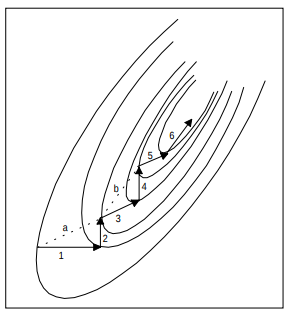
\includegraphics[width=0.33\linewidth]{powell_diagrama.png}
  \caption{Uma ilustração da maneira que o Algoritmo de Powell percorre o espaço de busca -- Retirado de \cite{fletcher1964function}}
\end{figure}

Assim, tem-se:

\begin{equation}
\begin{split}
z = F(x) \text{\phantom{0}e\phantom{0}}\phantom{0}
X = 
\begin{pmatrix}
x
\\ 
y
\end{pmatrix} \in R^2
\end{split}
\end{equation}

Na figura anterior, têm-se que as direções $1$ e $2$ são as da base inicial. A direção $a$ é a conjugada desta primeira iteração e substituirá a direção $1$ da base inicial. Minimiza-se então as direções da nova base, formando-se então a direção conjugada $b$, que substituirá a direção $2$ da base inicial. O processo é repetido até a condição de parada ser atingida.

\subsection{Evolução Diferencial}
O algoritmo de Evolução Diferencial proposto por \cite{storn1997differential} trabalha com uma população de
soluções iniciais, geradas aleatoriamente do espaço de busca $X_t = {x_{t_,i} | i = 1, ... , N_p}$ onde $x_{t,i}$ representa o i-ésimo indivíduo da t-ésima geração e $N_p$ o número de indivíduos da população. Um indíviduo é descrito como um vetor da forma:

\begin{equation}
\begin{split}
x_{t,i} = (x_{t,i,1}, x_{t,i,2}, ..., x_{t,i,n}) 
\end{split}
\end{equation}

onde $n$ é o número de variáveis de projeto. O algoritmo utiliza um processo de busca constituído na diferença entre duas soluções escolhidas aleatoriamente dentre as presentes na população. O
resultado é adicionado a uma terceira solução $x_{t,r_1}$ (estratégia \textit{best1bin}).


\begin{equation}
\begin{split}
v_{t,i} = x_{t,r_1} + F(x_{t,r_2} - x_{t,r_1})
\end{split}
\end{equation}

Onde $r_1 \neq r_2 \neq r_3$ e $F$ é o fator de escala multiplicado pelo
vetor diferença, $v_{t,i}$ é a $i\text{-esima}$ solução mutante da $t\text{-esima}$ geração e $x_{t,r_1}$ é o
vetor base no qual se aplica a mutação diferencial.\newline

Assim, obtém-se uma população mutante $V_{t} = {v_{t,i} | i = 1, 2, ..., N_p}$ que será recombinada com a população corrente $X_t$, formando a população de descendentes, chamada de $U_t$. 

\begin{equation}
\begin{split}
u_{t,i,j} = 
\left\{\begin{matrix}
v_{t,i,j} & \text{se } U_{[0,1]} \leq CR \text{\phantom{0}ou\phantom{0}} j = \delta_i \\
x_{t,i,j} & \text{caso contrário}
\end{matrix}\right.
\end{split}
\end{equation}

Em que $CR$ é o parâmetro de recombinação discreta, tal que $CR \in [0,1]$ e $\delta_i \in [1, ..., n]$ é sorteado aleatoriamente, garantindo que ao menos uma variável da solução teste passe para a solução descendente. Observa-se que o parâmetro $CR$ é capaz de administrar a porcentagem de $v_{t,i}$ herdada por $u_{t,i}$. Além disso, destaca-se que há um vetor mutante $u_{t,i,j}$ para cada indivíduo $x_{t,i,j}$ da população corrente. Logo ambas as populações, $X_t$ e $U_t$ possuem o mesmo número de indivíduos.\newline


Após gerada a população $U_t$,é realizada uma seleção entre as soluções das populações $X_t$ e $U_t$, avaliando o valor da função objetivo de $u_{t,i}$ e sua correspondente $x_{t,i}$,sendo aprovada a com melhor valor. A solução aprovada é classificada para compor a população corrente da próxima geração, $X_{t+1}$.
Neste caso, representa-se por um problema de maximização.

\begin{equation}
\begin{split}
x_{t+1,i} = 
\left\{\begin{matrix}
u_{t+1,i} & \text{se\phantom{0}} f(u_{t,i}) > f(x_{t,i}), \\
x_{t,i} & \text{caso contrário}
\end{matrix}\right.
\end{split}
\end{equation}

A ilustração abaixo representa como o algoritmo de Evolução Diferencial gera novos candidatos e percorre o espaço de busca:

\begin{figure}[H]
  \centering
  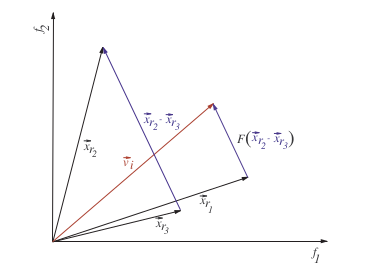
\includegraphics[width=0.5\linewidth]{ed_diagrama.png}
  \caption{Uma ilustração da maneira que o Algoritmo de Evolução Diferencial percorre o espaço de busca -- Adaptado de \cite{storn1997differential}}
\end{figure}

A população inicial é criada por amostragem do hipercubo latino, a fim de que todos os candidatos cubram o espaço de busca, de tal forma que que grandes áreas do espaço de busca possam ser avaliadas.
\subsection{Enxame de Partículas (PSO)}
Otimização por Enxame de Partículas, do inglês Particle Swarm Optimization (PSO), é uma técnica de computação evolucionária inspirada na simulação de um sistema social. O algoritmo PSO (\cite{bai2010analysis}) simula a migração e agregação de um bando de aves procurando por comida, local seguro, etc. O bando de aves representa o conjunto de soluções, sendo cada ave uma solução e, o local com o recurso buscado representa a função objetivo do problema de otimização. As possíveis soluções, i.e: as partículas, percorrem o espaço de busca, seguindo as melhores posições encontradas até o momento pelas próprias partículas e por todo o bando à procura do alvo (x ótimo). Estas melhores posições, as quais as partículas procuram seguir, podem ser classificadas tanto como a melhor posição encontrada por ela mesma até o momento, chamada $p_{\text{best}}$ ou como a melhor posição encontrada por toda a população levando em consideração todas as partículas, chamada $g_{\text{best}}$. Ao final da execução, a melhor ou as melhores soluções de acordo com uma função objetivo são apresentadas como resultado.
O PSO clássico, para N partículas, é dado por:

\begin{equation}
\begin{split}
v_{i}^{k+1} = & w v_{i}^{k} + c_1 \text{\phantom{0}} rand_{1} (p_{\text{best}} - x_{i}^{k}) + c_2 \text{\phantom{0}} rand_{2} (g_{\text{best}} - x_{i}^{k}) \\
x_{i}^{k+1} = & x_{i}^{k} + v_{i}^{k+1}
\end{split}
\end{equation}

\begin{figure}[H]
  \centering
  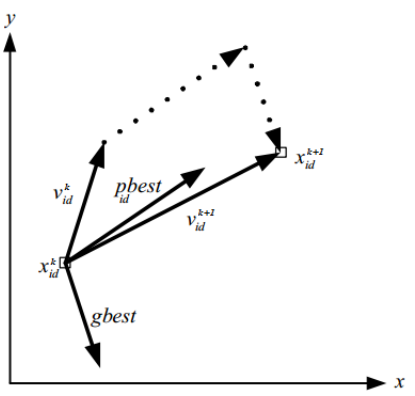
\includegraphics[width=0.5\linewidth]{pso_diagrama.png}
  \caption{Uma ilustração da maneira que o PSO percorre o espaço de busca}
\end{figure}

Onde $v_{id}^{k}$ representa a velocidade atual da partícula $x_{i}^{k}$. 
A velocidade adquirida pela partícula à cada iteração é determinada 
pela composição de sua velocidade atual com sua posição em relação à sua melhor posição e à melhor
posição do bando. \newline

A velocidade da partícula indica a direção que esta deve tomar, a fim de se aproximar do ótimo local ou global. Logo, a posição da partícula em cada iteração $x_{i}^{k+1}$ é a sua posição anterior mais sua velocidade atualizada $v_{i}^{k+1}$. Os termos $\text{rand}_{1}$ e $\text{rand}_{2}$ são números aleatórios uniformemente distribuídos no intervalo $[0, 1]$. \newline

A inércia da partícula, representada por $w$, introduz a preferência da partícula em continuar se movendo na mesma direção que seguia na iteração anterior. Um valor de inércia alto facilita uma exploração mais global, enquanto um valor baixo facilita uma exploração mais local na busca pelo ótimo (\cite{miranda2018pyswarms}).\newline

Os valores indicados por $c_1$ e $c_2$ são constantes positivas inteiras que correspondem a componentes cognitivas e sociais do bando, isto é, são parâmetros de confiança que indicam o quanto uma partícula confia em si ($c_1$) e quanto ela confia no bando ($c_2$). Os parâmetros de confiança e de inércia devem ser ajustados de
acordo com o problema aplicado, pois são utilizadas para a atualização do vetor velocidade (\cite{miranda2018pyswarms}).
\section{Resultados}
Os problemas foram resolvido com o seguintes parâmetros:

\begin{itemize}
\item no problema 1 $x_0 = (1.0, 1.0)$, no problema 2 $x_0 = (45.0, 30.0, 5.0)$ -- Apenas para o método de Powell (chute inicial);
\item $\phi_p      = 0.5$       -- fator de escala saindo da melhor posição da partícula;
\item $\phi_g      = 0.5$       -- fator de escala para buscar saindo da melhor posição do enxame;
\item minfunc   $= 10^{-8}$     -- menor mudanca na funcao objetivo que termina;
\item minstep   $= 10^{-8}$     -- tamanho de passo minimo da melhor posicao do enxame antes que a busca termine;
\item ${max}_{it}   = 100$      -- máximo de iterações;
\item $\omega     = 0.5$        -- Fator de escala da velocidade da partícula;
\item $N = 100$                 -- tamanho da população;
\item $r = 0.7$                 -- Probabilidade de recombinação no DE;
\item estratégia = best1bin     -- Estratégia de mutação do DE;
\item mutação   $= (0.5, 1)$  --  Taxa de Mutação do DE;
\end{itemize}

\subsection{Problema 1}


Foram obtidos os seguintes resultados:

\begin{longtable}[c]{|l|l|l|l|l|l|}
\hline
Powell - x                  & Powell - f(x)   & DE - x                      & DE - f(x)       & PSO - x                     & PSO - f(x)      \\ \hline
\endfirsthead
%
\multicolumn{6}{c}%
{{\bfseries Continuação da tabela \thetable\ da página anterior}} \\
\hline
Powell - x                  & Powell - f(x)   & DE - x                      & DE - f(x)       & PSO - x                     & PSO - f(x)      \\ \hline
\endhead
%
{[}0.00521 0.02836{]} & -0.10669 & {[}0.00521  0.028375{]} & -0.10669 & {[}0.00521 0.02837{]} & -0.10669 \\ \hline
\caption{Resultados do problema 1}
\label{tab:problema1}\\
\end{longtable}

Ou seja, o deslocamento $(u,v)$ para o sistema em equílibrio foi de aproximadamente $5.21 mm$ e $28.37 mm$, minimizando o sistema para uma energia potencial total de $-0.106 J$. Para atingir a convergência, foram necessárias respectivamente 6, 31 e 39 iterações para o algoritmo de Powell, DE e PSO. Abaixo, observa-se a convergência de cada algoritmo até o mínimo da função:

\begin{figure}[H]
\centering
\begin{subfigure}{0.5\textwidth}
  \centering
  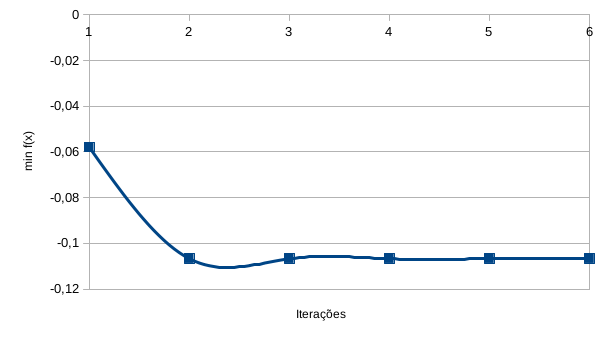
\includegraphics[width=\linewidth]{problema1_powell.png}
  %\caption{A subfigure}
\end{subfigure}%
\begin{subfigure}{0.5\textwidth}
  \centering
  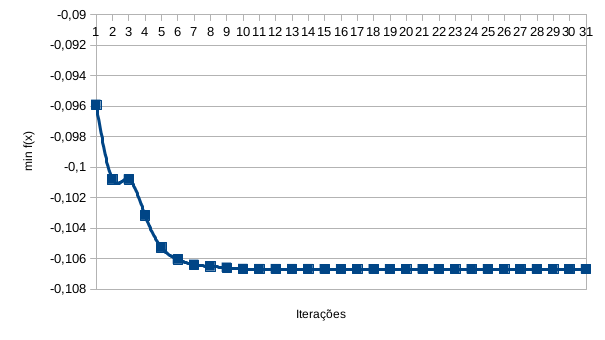
\includegraphics[width=\linewidth]{problema1_de.png}
  %\caption{A subfigure}
\end{subfigure}
\begin{subfigure}{0.5\textwidth}
  \centering
  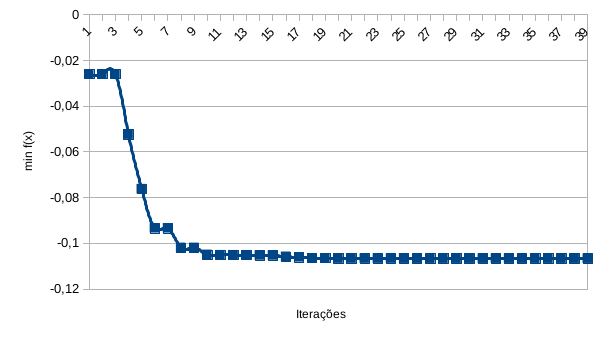
\includegraphics[width=\linewidth]{problema1_pso.png}
  %\caption{A subfigure}
\end{subfigure}
\caption{Convergência dos algoritmos Powell, DE e PSO testados}
\label{fig:p1}
\end{figure}
\subsection{Problema 2}

Visto que o problema 2 contém restrições de igualdade, foi necessária a reescrita da função objetivo através do Método da Penalidade Exterior, a fim de que as restrições de igualdade fossem incorporadas na função objetivo irrestrita. Devido a este fato, foi analisado o $rP$ (termo que pondera o valor da restrição sobre a função objetivo) da função objetivo a cada execução. Foram obtidos os seguintes resultados:

% Please add the following required packages to your document preamble:
% \usepackage{longtable}
% Note: It may be necessary to compile the document several times to get a multi-page table to line up properly
\begin{longtable}[c]{|l|l|l|l|}
\hline
Rp                     & Powell - x                                & Powell - f(x)  & Powell - g(x) \\ \hline
\endfirsthead
%
\multicolumn{4}{c}%
{{\bfseries Table \thetable\ continued from previous page}} \\
\hline
Rp                     & Powell - x                                & Powell - f(x)  & Powell - g(x) \\ \hline
\endhead
%
10\textasciicircum{}6  & {[} 0,55327702  0,07095995 -0,64445376{]} & -29502,421989  & 0,3196        \\ \hline
10\textasciicircum{}7  & {[} 0,39977555  0,0271785  -0,51592805{]} & -23723,9220183 & 0,0398        \\ \hline
10\textasciicircum{}8  & {[} 0,3757454   0,02229681 -0,49196887{]} & -22928,3090233 & 0,0041        \\ \hline
10\textasciicircum{}9  & {[} 0,37198841  0,02318257 -0,49028164{]} & -22843,3284124 & 0,0004        \\ \hline
10\textasciicircum{}10 & {[} 0,36858273  0,02707374 -0,49263702{]} & -22832,7967119 & 0,0001        \\ \hline
10\textasciicircum{}11 & {[}-0,43345571  0,34622668 -0,00501443{]} & 9929,79028962  & 0             \\ \hline
10\textasciicircum{}12 & {[}-0,43346566  0,34621875 -0,00499285{]} & 9930,65710977  & 0             \\ \hline
10\textasciicircum{}13 & {[}-0,43346665  0,34621795 -0,00499069{]} & 9930,7444071   & 0             \\ \hline
10\textasciicircum{}14 & {[}-0,43346672  0,34621787 -0,00499051{]} & 9930,75135866  & 0             \\ \hline
10\textasciicircum{}15 & {[}-0,43346673  0,34621786 -0,00499049{]} & 9930,75237759  & 0             \\ \hline
10\textasciicircum{}16 & {[}-0,43346673  0,34621786 -0,00499048{]} & 9930,75247955  & 0             \\ \hline
10\textasciicircum{}17 & {[}-0,43346673  0,34621786 -0,00499048{]} & 9930,75248946  & 0             \\ \hline
10\textasciicircum{}18 & {[}-0,43346673  0,34621786 -0,00499048{]} & 9930,75249037  & 0             \\ \hline
10\textasciicircum{}19 & {[}-0,43346673  0,34621786 -0,00499048{]} & 9930,75249046  & 0             \\ \hline
10\textasciicircum{}20 & {[}-0,43346673  0,34621786 -0,00499048{]} & 9930,75249047  & 0             \\ \hline
10\textasciicircum{}21 & {[}-0,43346673  0,34621786 -0,00499048{]} & 9930,75249047  & 0             \\ \hline
\caption{Soluções obtidas via algoritmo de Powell}
\label{tab:powell-p2}\\
\end{longtable}

% Please add the following required packages to your document preamble:
% \usepackage{longtable}
% Note: It may be necessary to compile the document several times to get a multi-page table to line up properly
\begin{longtable}[c]{|l|l|l|}
\hline
DE - x                                                & DE - f(x)     & DE - g(x) \\ \hline
\endfirsthead
%
\multicolumn{3}{c}%
{{\bfseries Table \thetable\ continued from previous page}} \\
\hline
DE - x                                                & DE - f(x)     & DE - g(x) \\ \hline
\endhead
%
{[}-6,48035531e-13  1,18662181e-01 -4,99048000e-03{]} & 1240,02479562 & 362       \\ \hline
{[}-0,41130483  0,34284927 -0,00499048{]}             & 9399,85000118 & 0,0321    \\ \hline
{[}-0,43132566  0,34593889 -0,00499048{]}             & 9878,37479558 & 0,0031    \\ \hline
{[}-0,43325332  0,34619049 -0,00499048{]}             & 9925,52159636 & 0,0003    \\ \hline
{[}-0,4334454   0,34621513 -0,00499048{]}             & 9930,22959866 & 0         \\ \hline
{[}-0,4334646   0,34621758 -0,00499048{]}             & 9930,70033246 & 0         \\ \hline
{[}-0,43346652  0,34621783 -0,00499048{]}             & 9930,74740518 & 0         \\ \hline
{[}-0,43346671  0,34621785 -0,00499048{]}             & 9930,75211278 & 0         \\ \hline
{[}-0,43346673  0,34621786 -0,00499048{]}             & 9930,75258324 & 0         \\ \hline
{[}-0,43346673  0,34621786 -0,00499048{]}             & 9930,75263024 & 0         \\ \hline
{[}-0,43346673  0,34621786 -0,00499048{]}             & 9930,75263498 & 0         \\ \hline
{[}-0,43346673  0,34621786 -0,00499048{]}             & 9930,75263542 & 0         \\ \hline
{[}-0,43346673  0,34621786 -0,00499048{]}             & 9930,75263546 & 0         \\ \hline
{[}-0,43346673  0,34621786 -0,00499048{]}             & 9930,75263555 & 0         \\ \hline
{[}-0,43346673  0,34621786 -0,00499048{]}             & 9930,75263549 & 0         \\ \hline
{[}-0,43346673  0,34621786 -0,00499048{]}             & 9930,7526357  & 0         \\ \hline
\caption{Soluções obtidas via Evolução Diferencial}
\label{tab:de-p2}\\
\end{longtable}

% Please add the following required packages to your document preamble:
% \usepackage{longtable}
% Note: It may be necessary to compile the document several times to get a multi-page table to line up properly
\begin{longtable}[c]{|l|l|l|l|}
\hline
Rp                     & PSO - x                                   & PSO - f(x)    & PSO - g(x) \\ \hline
\endfirsthead
%
\multicolumn{4}{c}%
{{\bfseries Table \thetable\ continued from previous page}} \\
\hline
Rp                     & PSO - x                                   & PSO - f(x)    & PSO - g(x) \\ \hline
\endhead
%
10\textasciicircum{}6  & {[} 0,          0,11866258 -0,00499048{]} & 1240,02479734 & 362        \\ \hline
10\textasciicircum{}7  & {[}-0,41130508  0,34284941 -0,00499048{]} & 9399,85000379 & 0,0321     \\ \hline
10\textasciicircum{}8  & {[}-0,4313257   0,34593893 -0,00499048{]} & 9878,3747961  & 0,0031     \\ \hline
10\textasciicircum{}9  & {[}-0,43325333  0,3461905  -0,00499048{]} & 9925,52159715 & 0,0003     \\ \hline
10\textasciicircum{}10 & {[}-0,4334454   0,34621511 -0,00499048{]} & 9930,22960282 & 0          \\ \hline
10\textasciicircum{}11 & {[}-0,4334646   0,34621759 -0,00499048{]} & 9930,70033397 & 0          \\ \hline
10\textasciicircum{}12 & {[}-0,43346653  0,34621783 -0,00499048{]} & 9930,74741237 & 0          \\ \hline
10\textasciicircum{}13 & {[}-0,43346671  0,34621785 -0,00499048{]} & 9930,75212868 & 0          \\ \hline
10\textasciicircum{}14 & {[}-0,43346673  0,34621785 -0,00499048{]} & 9930,75259885 & 0          \\ \hline
10\textasciicircum{}15 & {[}-0,43346674  0,34621786 -0,00499048{]} & 9930,75351379 & 0          \\ \hline
10\textasciicircum{}16 & {[}-0,43346674  0,34621786 -0,00499048{]} & 9930,75962469 & 0          \\ \hline
10\textasciicircum{}17 & {[}-0,43346674  0,34621786 -0,00499048{]} & 9930,98196715 & 0          \\ \hline
10\textasciicircum{}18 & {[}-0,43346674  0,34621786 -0,00499048{]} & 9930,95643021 & 0          \\ \hline
10\textasciicircum{}19 & {[}-0,43346672  0,34621785 -0,00499048{]} & 10035,0003305 & 0          \\ \hline
10\textasciicircum{}20 & {[}-0,43346674  0,34621787 -0,00499048{]} & 11399,7244991 & 0          \\ \hline
10\textasciicircum{}21 & {[}-0,43346674  0,34621786 -0,00499048{]} & 14915,491567  & 0          \\ \hline
\caption{Soluções obtidas via PSO}
\label{tab:pso-p2}\\
\end{longtable}

Os gráficos abaixo ilustram a convergência de cada algoritmo para um 

\begin{figure}[H]
\centering
\begin{subfigure}{0.5\textwidth}
  \centering
  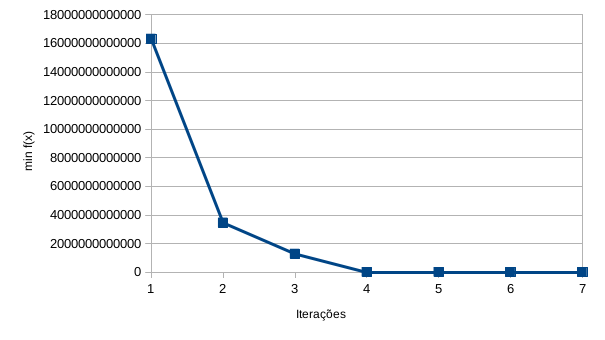
\includegraphics[width=\linewidth]{powell15.png}
  %\caption{A subfigure}
\end{subfigure}%
\begin{subfigure}{0.5\textwidth}
  \centering
  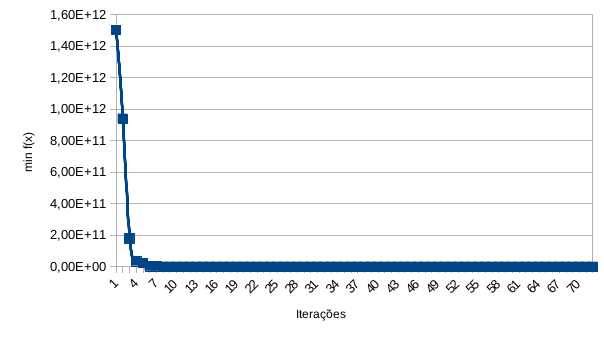
\includegraphics[width=\linewidth]{de15.png}
  %\caption{A subfigure}
\end{subfigure}
\begin{subfigure}{0.5\textwidth}
  \centering
  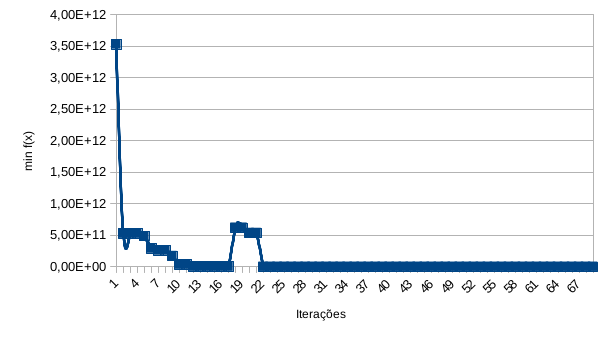
\includegraphics[width=\linewidth]{pso15.png}
  %\caption{A subfigure}
\end{subfigure}
\caption{Convergência dos algoritmos de Powell, Evolução Diferencial e PSO para $R_p = 10^{15}$}
\label{fig:p2}
\end{figure}

Ou seja, o vetor de ângulos $(\theta_1, \theta_2, \theta_3) \approx ((-24.83, 19.83, -0.28))$ uma vez que o sistema estiver em equilíbrio.
\section{Conclusão}
O príncipio do mínimo da energia potencial é uma formulação interessante que permite que vários problemas físicos em contextos estáticos sejam resolvidos de maneira rápida e precisa. Este conceito foi aplicado em 2 problemas de mecânica, com um grau de não-linearidade substancial, e através de métodos de otimização estocásticos irrestritos, foram obtidas soluções para os mesmos. Nota-se que o algoritmo de Evolução Diferencial é capaz de convergir para uma solução dentro da faixa de tolerância a partir de populações menores, diferentemente do PSO. Apesar da robustez dos algoritmos estocásticos é evidente que seu custo computacional é extremamente custoso quando comparado a métodos clássicos. Além disso, todos os algoritmos necessitam de uma escolha minuciosa do termo $Rp$ em casos onde há restrições no problema, visto que todos os algoritmos avaliados respeitaram as restrições apenas para $Rp > 10^{11}$. O PSO por sua vez começou a divergir do x ótimo após um $Rp > 10^{18}$\newline
Concluí-se que o algoritmo de Evolução Diferencial é o mais apto para resolução de problemas de minimização da energia potencial total de sistemas em casos onde é garantido que o espaço de busca esteja igualmente populado pelos vetores iniciais (algo alcançável através da amostragem por hipercubo latino).
\bibliographystyle{apalike}
\bibliography{sample}
\end{document}